\documentclass{cumcmthesis}
    %\documentclass[withoutpreface,bwprint]{cumcmthesis} %去掉封面与编号页

    \title{龙门吊问题的数学建模}
    \tihao{A}            % 题号
    \baominghao{042}    % 报名号
    \schoolname{武汉大学}
    \membera{周澳}
    \memberb{傅宇千}
    \memberc{刘志豪}
    \supervisor{指导老师}
    \yearinput{2020}     % 年
    \monthinput{08}      % 月
    \dayinput{15}        % 日

\begin{document}
\maketitle
\begin{abstract}
    摘要的具体内容。
    \keywords{关键词1\quad  关键词2\quad   关键词3}
\end{abstract}
\tableofcontents
\section{问题重述}
\subsection{问题的提出}
\section{符号说明}
\begin{center}
    \begin{tabular}{cc}
        \hline
        \makebox[0.3\textwidth][c]{符号} & \makebox[0.4\textwidth][c]{意义} \\ \hline
        D                                & 木条宽度(cm)                   \\ \hline
    \end{tabular}
\end{center}
\section{问题分析}
题目给出的龙门吊问题可以看作二维的质点运动问题,
\section{模型假设}
\section{建立模型}
\subsection{货物运动的动力学模型}
如图所示建立坐标系:

\centerline{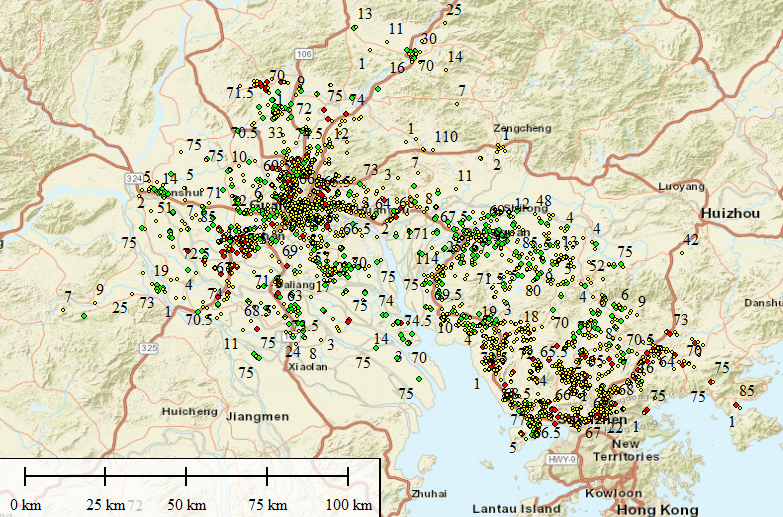
\includegraphics[width=10cm]{1.png}}
设吊车位置坐标为$x_a$,速度为$v_a$;货物的位置$(x,y)$,速度$v$,水平速度$v_{x}$,缆绳与竖直方向的角度为$\theta$(顺时针为正)。令$T_1=t_1,\quad T_2=t_1+t_2,\quad T_3=t_1+t_2+t_3,\quad T_4=t_1+t_2+t_3+t_4$。吊绳能承受的最大拉力$T_{max}=20000g,\quad g$取$9.8m/s^2$。

取货物为研究对象,用分析力学方法,取广义坐标$\theta$

(1)当$0 \leq t \leq T_1$时,吊车匀加速运动,对于货物有如下拉格朗日函数:
$$L_{1}=\frac{m}{2}\left(l^{2} \dot{\theta}^{2}-2 a l \dot{\theta} t \cos \theta+a^{2} t^{2}\right)+m gl\cos \theta$$

代入拉格朗日方程$$\frac{d}{d t}\left(\frac{\partial L_{1}}{\partial \dot{\theta}}\right)-\frac{\partial L_1}{\partial \theta}=0$$

得到运动微分方程:$$l \ddot{\theta}+a \dot{\theta} t \sin \theta-a \cos \theta+g \sin \theta=0$$
$$\text{初始条件}\left.\theta\right|_{t=0}=0,\left.\quad \dot{\theta}\right|_{t=0}=0$$

由$\theta(t),0 \leqslant t \leqslant T_{1}$,有

$$\left\{\begin{array}{l}
        x=x_{a}-l \theta \sin \theta=\frac{a}{2} t^{2}-\operatorname{lsim} \theta \\
        v_{x}=v_{a}-l \dot{\theta} \cos \theta=a t-l \dot{\theta} \cos \theta
    \end{array}\right.$$

(2)当$T_1 \leq t \leq T_2$时,吊车匀速运动,对于货物同上可得运动微分方程:
$$\ddot{\theta}+\frac{g}{l} \sin \theta=0$$
$$\text{初始条件}\left \{\begin{array}{l}
        \left.\theta\right|_{t=T_{1}^{+}}=\left.\theta\right|_{t=T_{1}^{-}} \\
        \left.\dot{\theta}\right|_{t=T_{1}^{+}}=\left.\dot{\theta}\right|_{t=T_{1}^{-}}
    \end{array}\right.$$

此时有:$$\left\{\begin{array}{l}
        x=x_{a}-l\theta \sin \theta=\frac{a}{2} T_{1}^{2}+aT_1(t-T_1)-l\sin \theta \\
        v_{x}=v_{a}-l \dot{\theta} \cos \theta=a T_{1}-l\dot{\theta }\cos \theta
    \end{array}\right.$$

(3)当$T_2 \leq t \leq T_3$时,吊车匀减速运动,对于货物同(1)可得运动微分方程:
$$l \ddot{\theta}+a\left(T_{1}+T_{2}-t\right) \dot{\theta} \sin \theta+a \cos \theta+g \sin \theta=0$$
$$\text{初始条件}\left \{\begin{array}{l}
        \left.\theta\right|_{t=T_{2}^{+}}=\left.\theta\right|_{t=T_{2}^{-}} \\
        \left.\dot{\theta}\right|_{t=T_{2}}=\left.\dot{\theta}\right|_{t=T_{2}^{-}}
    \end{array}\right.$$
此时有:$$\left\{\begin{array}{l}
        v_{x}=a\left(T_{1}+T_{2}-t\right)-l \dot{ \theta} \cos \theta \\
        x=x_{2}+aT_{1}(t-T_{2})-\frac{a}{2}(t-T_{2})^{2}-l\sin\theta
    \end{array}\right.$$

(4)当$T_3 \leq t \leq T_4$时,吊车匀速运动,对于货物同(1)可得运动微分方程:
$$\ddot{\theta}+\frac{g}{l} \sin \theta=0$$
$$\text{初始条件}\left \{\begin{array}{l}
        \left.\theta\right|_{t=T_{3}^{+}}=\left.\theta\right|_{t=T_{3}^{-}} \\
        \left.\dot{\theta}\right|_{t=T_{3}^{+}}=\left.\dot{\theta}\right|_{t=T_{3}^{-}}
    \end{array}\right.$$
此时有:$$\left\{\begin{array}{l}
    v_{x}=a\left(T_1+T_{2}-T_{3}\right)-l \dot{\theta} \cos \theta \\
    x=x_{3}+a\left(T_{1}+T_{2}-T_{3}\right)\left(t-T_{3}\right)-l \sin \theta
    \end{array}\right.$$

整个过程中的最大摆角$\theta_{\max }=\max \theta(t), \quad 0 \leqslant t \leqslant T_{4}$,

对于货物最终的水平速度,取第四段匀速过程中货物水平速度绝对值的最大值$v_{4xmax}=max\left \{v_{x},T_3 \leq t \leq T_4\right \}$,要求$v_{4max} \leq 0.5m/s$。

运动全过程中货物的竖直速度$v_{y}=-l\dot{\theta}\sin\theta,\quad 0\leq t\leq T_4$,对速度求导可得水平、竖直方向的加速度,由此可以计算整个运动过程中每一时刻的拉力:$$\left\{\begin{array}{l}
    F_{x}=m a_{x} \\
    F_{y}=mg-ma_{y}
    \end{array}\right.$$
要求$F \leq F_{max},0 \leq t \leq T_4$
\subsection{对摆角、效率的优化模型}


\section{模型求解}
\section{模型检验}
\section{总结与推广}
\begin{thebibliography}{9}%宽度9
    \bibitem{bib:one} ....
\end{thebibliography}
\begin{appendices}
    附录的内容。
\end{appendices}
\end{document}